\subsection{OpenMP Affinity Settings}
As explained in Section~\ref{sec:intro} OpenMP 4.0 provides two environment variables OMP\_PROC\_BIND and OMP\_PLACES to help users define the thread placement for their shared memory OpenMP application. We experiment with the two flavors of the Jacobi program to observe the behavior over \textit{(a)} under-subscribed socket, \textit{(b)} fully-subscribed socket and \textit{(c)} across-socket utilization of CPUs. The \textit{numactl} hardware characteristics for Crest is as shown in Figure~\ref{fig:crest}

\begin{figure}[h]
  \centering
  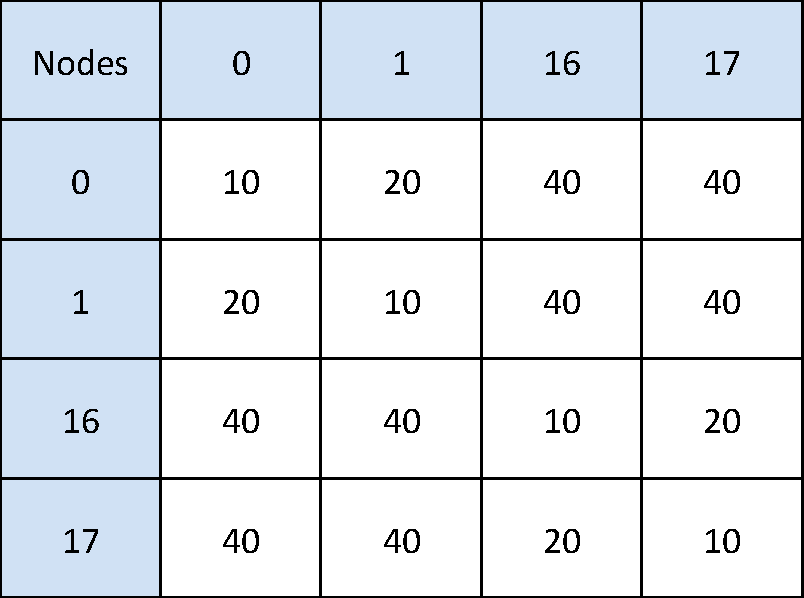
\includegraphics[height=0.3\textwidth]{./Images/crest.pdf}
       \caption{\textit{Numactl} hardware characteristics of Crest}
       \label{fig:crest}
\end{figure}
%
\begin{figure}[!h]
    \centering
    \begin{subfigure}[b]{0.5\textwidth}
        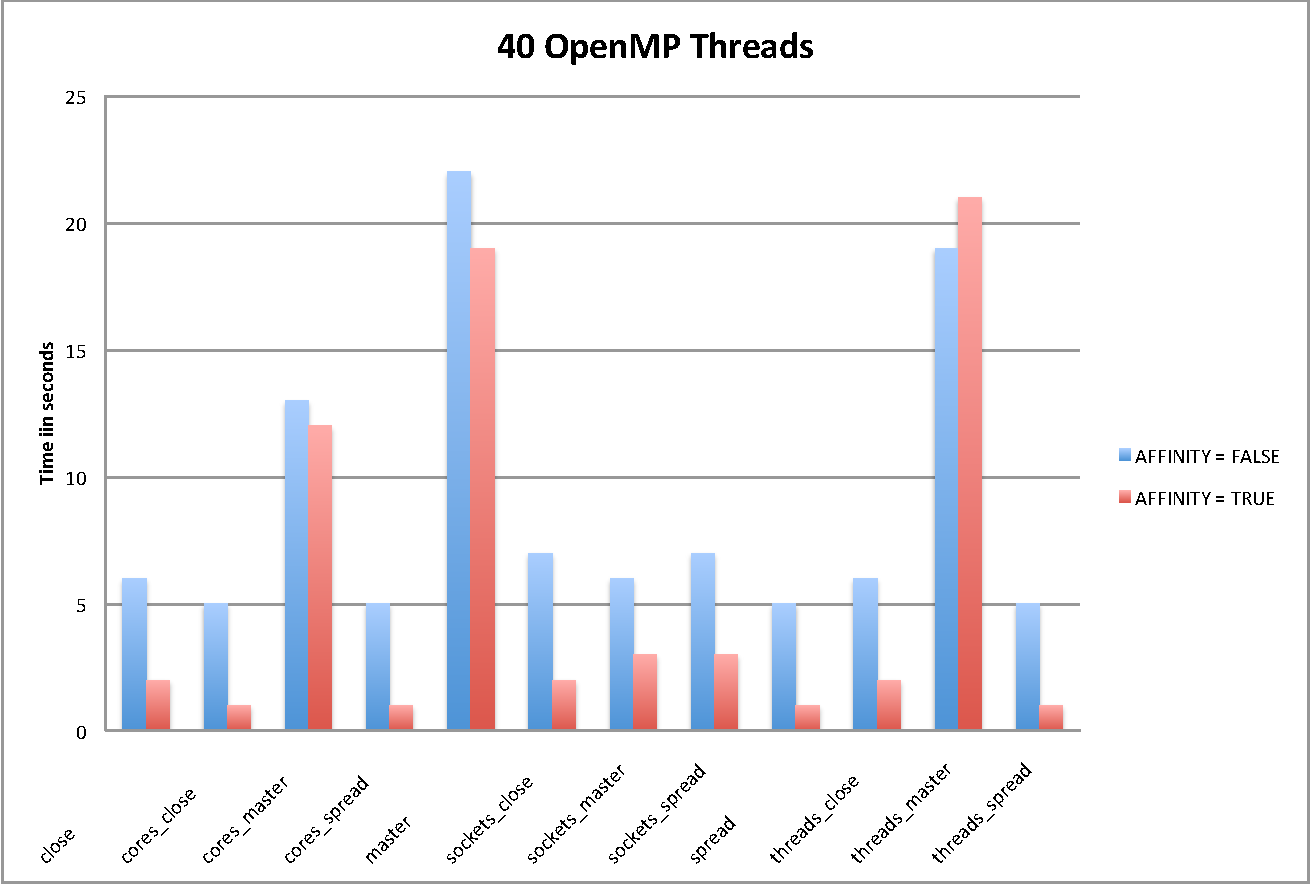
\includegraphics[width=\textwidth]{./Images/J40_time_bar}
        \caption{Partially utilized socket - 40 OpenMP threads configuration}
        \label{fig:J40}
    \end{subfigure}
  
    \begin{subfigure}[b]{0.5\textwidth}
        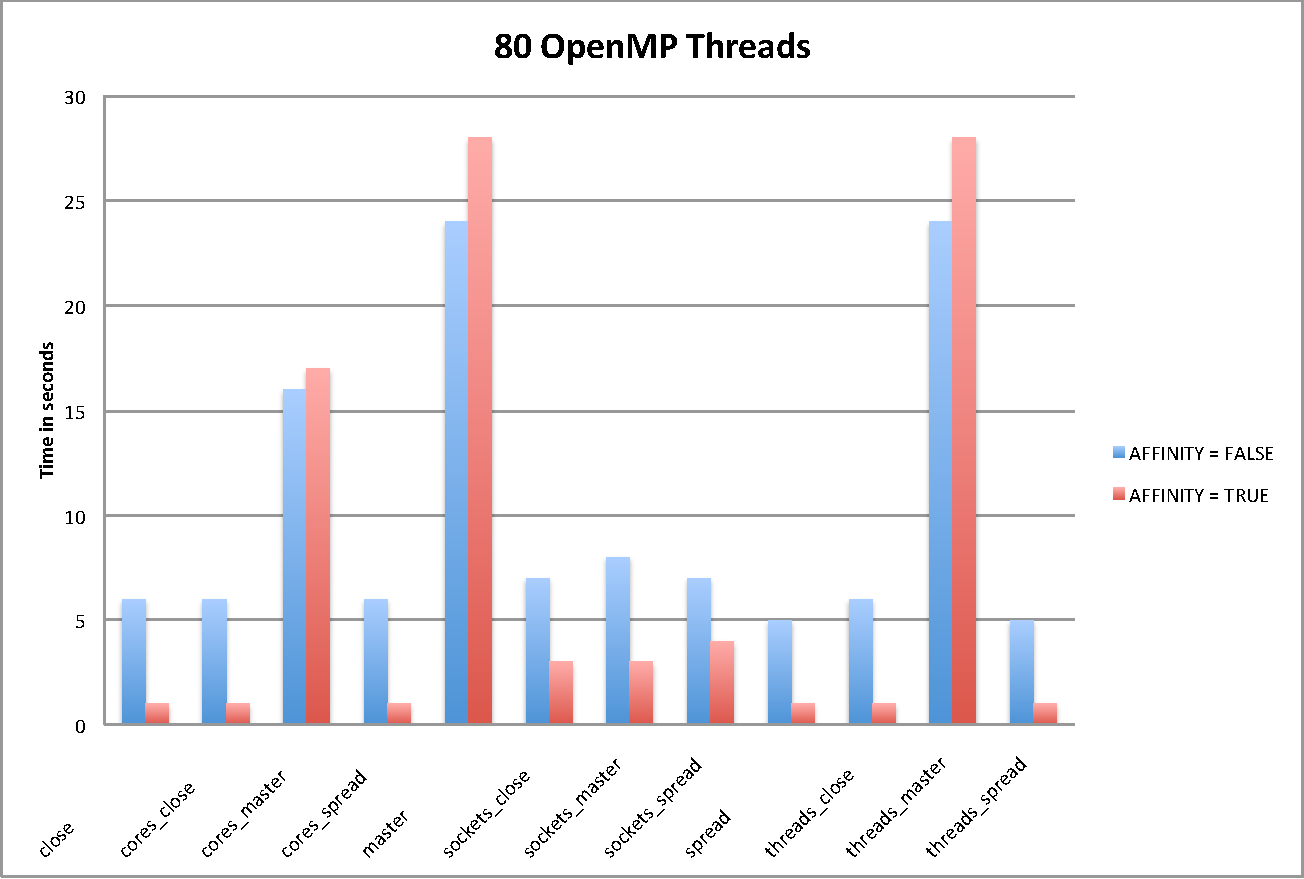
\includegraphics[width=\textwidth]{./Images/J80_time_bar}
        \caption{Fully utilized socket - 80 OpenMP threads configuration}
        \label{fig:J80}
    \end{subfigure}
  
      \begin{subfigure}[b]{0.5\textwidth}
        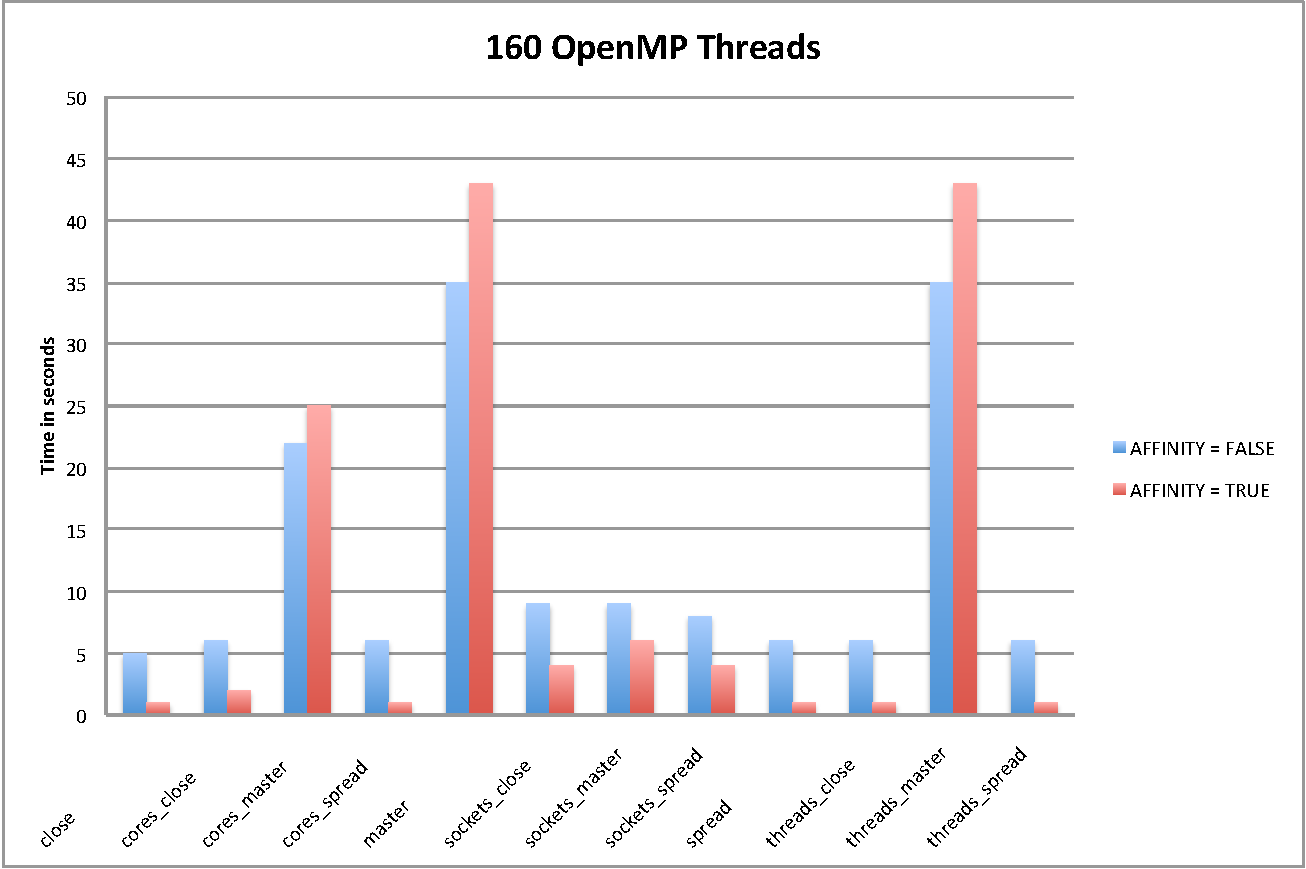
\includegraphics[width=\textwidth]{./Images/J160_time_bar}
        \caption{Across socket CPU utilization - 160 OpenMP threads configuration}
        \label{fig:J160}
    \end{subfigure}
    \caption{Timing for Jacobi program with and without data-affinity}\label{fig:Jacobi}
\end{figure}